\lstdefinelanguage{plaintext}{
  sensitive=false,
  comment=[l]{//},
  morecomment=[s]{/*}{*/},
  identifierstyle=\color{black},
  morestring=[b]',
  morestring=[b]"
}

\lstset
{ 
    language=plaintext,
    basicstyle=\footnotesize,
    numbers=left,
    stepnumber=1,
    showstringspaces=false,
    tabsize=1,
    breaklines=true,
    breakatwhitespace=false,
    frame=leftline
}

\chapter{Perancangan}
\label{chap:Perancangan}

Pada bab ini dibahas mengenai perancangan perangkat lunak yang dibangun, meliputi perancangan kelas dan algoritma pengecekan dokumen skripsi.

\section{Perancangan Kelas}
Pada bagian ini akan dijelaskan rancangan kelas yang akan digunakan pada perangkat lunak. Rancangan kelas tersebut akan ditunjukan oleh diagram kelas di bawah ini:

\begin{figure}[H]
	\centering	
	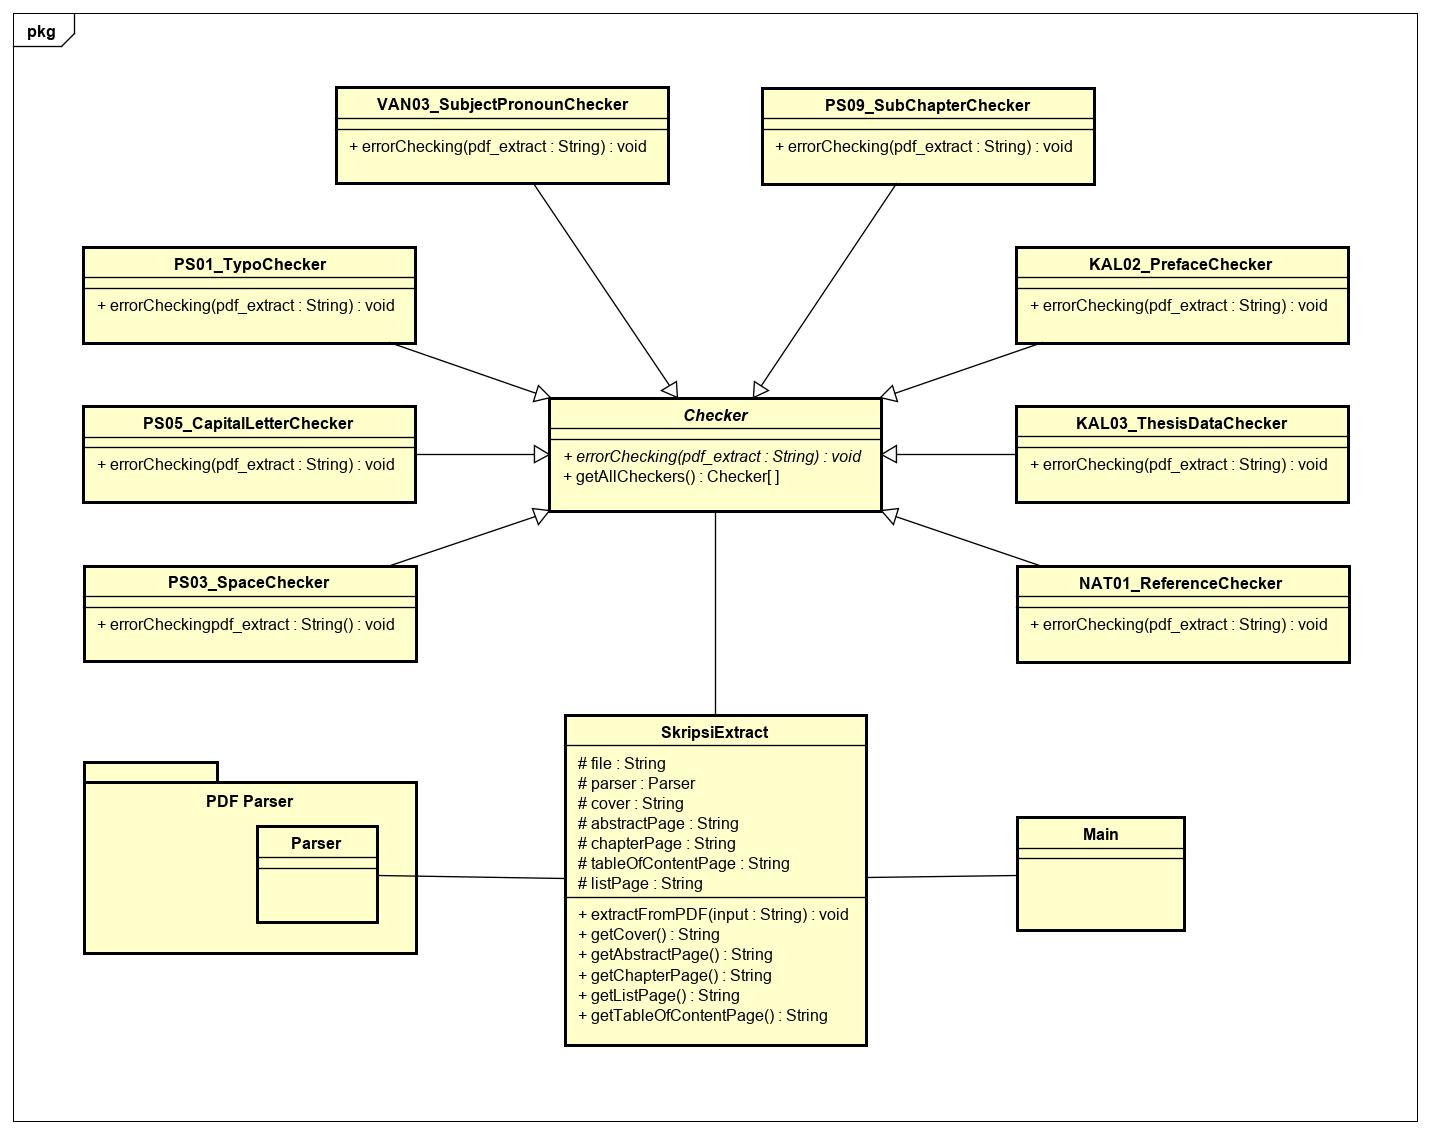
\includegraphics[scale=0.44]{class-diagram.png}
	\caption{Diagram kelas Aplikasi Pemeriksa Kesalahan Dokumen Skripsi}	
	\label{fig:diagram_kelas} 
\end{figure}

Pada gambar \ref{fig:diagram_kelas} telah ditunjukan bahwa perangkat lunak memiliki sebelas kelas dan sebuah \textit{library PDF Parser}. Rincian dari setiap kelas tersebut akan dijelaskan sebagai berikut:

\begin{enumerate}

	\item Kelas Checker \\
	Kelas ini merupakan kelas \textit{Parent} dari semua \textit{checker} yang akan diimplementasi pada perangkat lunak. Berikut adalah \textit{method} yang terdapat pada kelas ini:
	
		\begin{itemize}
			\item errorChecking(\$pdf\_extract) \\
			Method ini merupakan method abstrak, yang akan diturunkan kepada seluruh anak kelasnya. Method ini berfungsi untuk memeriksa kesalahan pada dokumen skripsi sesuai dengan peran yang diberikan pada kelas tersebut. Method ini menerima masukan pdf\_extract dengan tipe data kelas \textit{SkripsiExtract}. Parameter tersebut dapat digunakan oleh masing-masing kelas \textit{Checker} untuk memanggil \textit{method getter} yang diperlukan. Tidak semua pemeriksa memerlukan seluruh isi halaman dari dokumen skripsi.			
			
			\item getAllChecker() \\
			Method ini berfungsi untuk melakukan instansiasi seluruh anak kelas \textit{Checker}. Method ini mengembalikan hasil instansiasi anak kelas \textit{Checker}.
		\end{itemize}
	
	\item Kelas KAL02\_PrefaceChecker \\
	Kelas ini bertanggungjawab untuk memeriksa ada atau tidaknya kata pengantar sebelum memulai bab atau subbab. Berikut adalah \textit{method} yang terdapat pada kelas ini:
	
		\begin{itemize}
			\item errorChecking(\$pdf\_extract) \\
			Method ini berfungsi untuk memeriksa kesalahan pada dokumen skripsi. Method ini menerima masukan pdf\_extract dengan tipe data kelas \textit{SkripsiExtract}. Bagian yang diperiksa pada \textit{checker} ini hanya bab 1 hingga 6.
		\end{itemize}
	
	\item Kelas KAL03\_ThesisDataChecker \\
	Kelas ini bertanggungjawab untuk memeriksa kelengkapan data skripsi yang ditulis dalam bahasa Indonesia maupun bahasa Inggris. Berikut adalah \textit{method} yang terdapat pada kelas ini:
			
		\begin{itemize}
			\item errorChecking(\$pdf\_extract) \\
			Method ini berfungsi untuk memeriksa kesalahan pada dokumen skripsi. Method ini menerima masukan pdf\_extract dengan tipe data kelas \textit{SkripsiExtract}. Bagian yang diperiksa pada \textit{checker} ini adalah halaman cover bahasa Indonesia dan bahasa Inggris.
		\end{itemize}
		
	\item Kelas NAT01\_ReferenceChecker \\
	Kelas ini bertanggungjawab untuk memeriksa referensi yang akan dirujuk dalam dokumen. Berikut adalah \textit{method} yang terdapat pada kelas ini:
	
		\begin{itemize}
			\item errorChecking(\$pdf\_extract) \\
			Method ini berfungsi untuk memeriksa kesalahan pada dokumen skripsi. Method ini menerima masukan pdf\_extract dengan tipe data kelas \textit{SkripsiExtract}. Bagian yang diperiksa pada \textit{checker} ini adalah bab 1 hingga 6.
		\end{itemize}
			
	\item Kelas PS01\_TypoChecker \\
	Kelas ini bertanggungjawab untuk memeriksa kesalahan penulisan kata. Berikut adalah \textit{method} yang terdapat pada kelas ini:
	
		\begin{itemize}
			\item errorChecking(\$pdf\_extract) \\
			\textit{Method} ini berfungsi untuk memeriksa kesalahan pada dokumen skripsi. Method ini menerima masukan pdf\_extract dengan tipe data kelas \textit{SkripsiExtract}. Bagian yang diperiksa pada \textit{checker} ini adalah bab 1 hingga 6.
		\end{itemize}
			
	\item Kelas PS03\_SpaceChecker \\
	Kelas ini bertanggungjawab untuk memeriksa penggunaan spasi sebelum dan setelah tanda baca. Berikut adalah \textit{method} yang terdapat pada kelas ini:	
	
		\begin{itemize}
			\item errorChecking(\$pdf\_extract) \\
			\textit{Method} ini berfungsi untuk memeriksa kesalahan pada dokumen skripsi. Method ini menerima masukan pdf\_extract dengan tipe data kelas \textit{SkripsiExtract}. Bagian yang diperiksa pada \textit{checker} ini adalah bab 1 hingga 6.
		\end{itemize}
			
	\item Kelas PS05\_CapitalLetterChecker \\
	Kelas ini bertanggungjawab untuk memeriksa penggunaan huruf kapital pada awal kalimat. Berikut adalah \textit{method} yang terdapat pada kelas ini:
		
		\begin{itemize}
			\item errorChecking(\$pdf\_extract) \\
			\textit{Method} ini berfungsi untuk memeriksa kesalahan pada dokumen skripsi. Method ini menerima masukan pdf\_extract dengan tipe data kelas \textit{SkripsiExtract}. Bagian yang diperiksa pada \textit{checker} ini adalah bab 1 hingga 6.
		\end{itemize}
			
	\item Kelas PS09\_SubChapterChecker \\
	Kelas ini bertanggungjawab untuk memeriksa subbab yang ada dalam sebuah bab. Berikut adalah \textit{method} yang terdapat pada kelas ini:
			
		\begin{itemize}
			\item errorChecking(\$pdf\_extract) \\
			Method ini berfungsi untuk memeriksa kesalahan pada dokumen skripsi. Method ini menerima masukan pdf\_extract dengan tipe data kelas \textit{SkripsiExtract}. Bagian yang diperiksa pada \textit{checker} ini adalah bab 1 hingga 6.
		\end{itemize}
			
	\item Kelas VAN03\_SubjectProunounChecker \\
	Kelas ini bertanggungjawab untuk memeriksa penggunaan kata ganti orang pada dokumen skripsi. Berikut adalah \textit{method} yang terdapat pada kelas ini:
	
		\begin{itemize}
			\item errorChecking(\$pdf\_extract) \\
			Method ini berfungsi untuk memeriksa kesalahan pada dokumen skripsi. Method ini menerima masukan pdf\_extract dengan tipe data kelas \textit{SkripsiExtract}. Bagian yang diperiksa pada \textit{checker} ini adalah bab 1 hingga 6.
		\end{itemize}
			
	\item Kelas SkripsiExtract \\
	Kelas ini bertanggungjawab untuk melakukan ekstak file PDF skripi. Berikut adalah atribut yang terdapat pada kelas ini:
	
		\begin{itemize}
			\item file \\
			Atribut ini berfungsi untuk menyimpan nama file dari dokumen skripsi.
			
			\item parser \\			
			Atribut ini berfungsi sebagai instansiasi kelas Parser dari \textit{Library PDF Parser}.
			
			\item cover \\
			Atribut ini berfungsi untuk menyimpan hasil ekstrak dari halaman cover bahasa Indonesia dan bahasa Inggris.
			
			\item abstractPage \\			
			Atribut ini berfungsi untuk menyimpan hasil ekstrak dari halaman abstrak bahasa Indonesia dan bahasa Inggris.
			
			\item chapterPage \\	
			Atribut ini berfungsi untuk menyimpan hasil ekstrak mulai dari bab 1 hingga bab 6.
			
			\item listPage \\
			Atribut ini berfungsi untuk menyimpan hasil ekstrak pada halaman daftar isi, daftar tabel, daftar gambar dan daftar referensi.
			
		\end{itemize}
	
	Kelas ini juga memiliki \textit{method} yang berkaitan dengan proses ekstrak dokumen skripsi dan penyimpanan hasil ekstraknya. Berikut adalah \textit{method} yang terdapat pada kelas ini:
		
		\begin{itemize}
			\item extractFromPDF(\$input) \\
			Method ini berfungsi untuk melakukan proses ekstrak file PDF skripsi. Hasil dari ekstrak tersebut akan disimpan ke dalam beberapa bagian, seperti cover, halaman abstrak, dan sebagainya. 
			
			\item getCoverPage() \\
			Method ini berfungsi untuk mendapatkan halaman cover skripsi dalam bahasa Indonesia dan bahasa Inggris.
			
			\item getAbstractPage() \\
			Method ini berfungsi untuk mendapatkan halaman abstrak dalam bahasa Indonesia dan bahasa Inggris.
			
			\item getListPage() \\
			Method ini berfungsi untuk mendapatkan halaman daftar isi, daftar gambar, daftar tabel dan daftar referensi.
			
			\item getContent() \\
			Method ini berfungsi untuk mendapatkan halaman konten skripsi dari bab 1 sampai bab 6.
			
		\end{itemize}
	
	\item Kelas Main \\
	Kelas ini digunakan untuk menjalankan perangkat lunak. Kelas ini tidak memiliki atribut dan \textit{method}, hanya terdiri dari beberapa baris kode yang memanggil \textit{method} untuk mengekstrak dan memeriksa file PDF skripsi. 

\end{enumerate} 

\section{Perancangan Perangkat Lunak}
Pada bagian ini akan dijelaskan perancangan untuk mengekstrak dokumen skripsi dan pola pengecekan kesalahan yang akan digunakan pada perangkat lunak.
 
\subsection{Algoritma untuk Mengekstrak Dokumen}
Dokumen skripsi yang akan diperiksa dalam perangkat lunak merupakan file yang memiliki ekstensi \textit{PDF}. Perangkat lunak memerlukan ekstraksi dari \textit{PDF} agar dapat melakukan pemeriksaan. Perangkat lunak menggunakan \textit{library PDFParser} untuk mengekstrak dokumen skripsi. Pada \textit{library} tersebut, terdapat 2 metode yang digunakan untuk mengekstrak dokumen.
	
\begin{lstlisting}[caption={Potongan kode untuk mengesktrak seluruh halaman dokumen}	\label{lst:all_page},language=php,xleftmargin=.2\textwidth] 
include 'vendor/autoload.php';
	
$parser = new \Smalot\PdfParser\Parser();
$pdf    = $parser->parseFile('document.pdf');
$text   = $pdf->getText();
\end{lstlisting}
	
\begin{lstlisting}[caption={Potongan kode untuk mengesktrak halaman dokumen secara spesifik}
\label{lst:specific_page},language=php,xleftmargin=.2\textwidth] 
include 'vendor/autoload.php';

$parser = new \Smalot\PdfParser\Parser();
$pdf    = $parser->parseFile('document.pdf');
$pages  = $pdf->getPages();
\end{lstlisting}

Listing \ref{lst:all_page} dan listing \ref{lst:specific_page} merupakan potongan kode yang terdapat pada dokumentasi \textit{library PDF Parser}. Kode dari kedua listing tersebut hampir mirip, yang menjadi pembeda adalah pada baris ke-5. Listing \ref{lst:all_page} menggunakan \textit{method getText()} dan hasil dari ekstraknya disimpan menjadi sebuah kesatuan dari halaman awal hingga halaman akhir. Listing \ref{lst:specific_page} menggunakan \textit{method getPages()} dan hasil dari ekstraknya disimpan dalam sebuah array String sejumlah halaman yang ada pada dokumen.

Pada skripsi ini akan digunakan metode yang mengesktrak halaman-halaman secara spesifik. Hasil ekstrak akan disimpan dalam beberapa bagian, berdasarkan konten-konten yang ada. Konten-konten yang dimaksud seperti, halaman cover, abstrak, daftar isi, daftar tabel, daftar gambar dan seterusnya. Ada beberapa alasan yang mendorong untuk melakukan pemisahan konten-konten tersebut, salah satunya yaitu agar pemeriksa dapat memeriksa bagian-bagian spesifik yang menjadi tanggungjawab dari pemeriksa tersebut.

\subsection{Pola Pengecekan Kesalahan}
Hasil survei kesalahan-kesalahan dalam penulisan dokumen skripsi sudah disaring dan akan diimplementasikan dalam perangkat lunak. Pengecekan kesalahan tersebut akan dilakukan dengan menggunakan teknik \textit{pattern matching regex}. Hasil ekstrak dari PDF skripsi akan dipotong dengan delimiter karakter titik dan spasi 1 buah ke dalam sebuah array. Hal ini dilakukan agar pemeriksaan dapat lebih mudah dilakukan apabila teks sudah dipecah menjadi sebuah kalimat utuh. Berikut adalah rincian dari hasil survei yang dipilih beserta penyelesaiannya:

\begin{enumerate}
	\item Penulisan kata (PS-01) \\
	Untuk mendeteksi kesalahan penulisan kata, akan digunakan ekstensi kamus bahasa Indonesia \textit{LibreOffice}. Dengan digunakan kamus tersebut, kesalahan penulisan suatu kata dapat diminimalisir. Pola pengecekan yang digunakan akan dijelaskan pada tabel \ref{tab:ps01}.
		
	\begin{table}[H]
		\renewcommand{\arraystretch}{1.5}
		\caption {Tabel rincian pengecekan survei PS-01} 
		\label{tab:ps01}
		\begin{center}
			\begin{tabular}{|p{3.5cm} |p{10.5cm}|}
			\hline 
			Pola & / $\hat{}$ / \\ 
			\hline 
			Deskripsi & Pola akan mencocokan kata yang akan diperiksa dengan kamus bahasa Indonesia \textit{LibreOffice} \\ 
			\hline 
			Contoh & Istilah \textit{regex} berasal dari toeri matematika dan komputer sains, yang mencerminkan sifat ekspresi dalam matematika yang disebut keteraturan. \\ 
			\hline 
			Laporan & Pada baris ini ditemukan penulisan kata yang salah \\ 
			\hline
			\end{tabular}
		\end{center}
	\end{table}
	
	\item Pemberian spasi sebelum dan sesudah tanda baca (PS-03) \\
	Kesalahan ini akan terdeteksi apabila tidak ada karakter spasi sebelum ataupun sesudah tanda baca. Pola pengecekan yang digunakan akan dijelaskan pada tabel \ref{tab:ps03}.
		
	\begin{table}[H]
		\renewcommand{\arraystretch}{1.5}
		\caption {Tabel rincian pengecekan survei PS-03} 
		\label{tab:ps03}
		\begin{center}
			\begin{tabular}{|p{3.5cm} |p{10.5cm}|}
			\hline 
			Pola & /([A-Za-z0-9]*[,.!?][A-Za-z0-9])/ \\ 
			\hline 
			Deskripsi & Pola akan mendeteksi kesalahan apabila setelah tanda [,.!?] terdapat karakter spasi atau tidak \\ 
			\hline 
			Contoh & Aplikasi ini dijalankan melalui melalui terminal command Windows.laporan dari hasil kesalahan tersebut akan ditampilkan melalui terminal command Windows. \\ 
			\hline 
			Laporan & Perhatikan spasi sebelum atau setelah tanda baca \\ 
			\hline
			\end{tabular}
		\end{center}
	\end{table}
	
	\item Awal kalimat tidak menggunakan huruf kapital (PS-05) \\
	Kesalahan ini akan terdeteksi apabila setelah tanda baca pada akhir kalimat, karakter pertama setelah spasi menggunakan huruf kecil. Pola pengecekan yang digunakan akan dijelaskan pada tabel \ref{tab:ps05}.
		
	\begin{table}[H]
		\renewcommand{\arraystretch}{1.5}
		\caption {Tabel rincian pengecekan survei PS-05} 
		\label{tab:ps05}
		\begin{center}
			\begin{tabular}{|p{3.5cm} |p{10.5cm}|}
			\hline 
			Pola & / $\hat{}$ ($\backslash$s[a-z][a-z0-9].*)/ \\ 
			\hline 
			Deskripsi & Pola akan mendeteksi karakter pertama dalam sebuah kalimat yang menggunakan huruf kecil   \\ 
			\hline 
			Contoh & aplikasi sederhana ini, dapat dimanfaatkan oleh mahasiswa Informatika Unpar secara mandiri \\ 
			\hline 
			Laporan & Huruf pertama pada kalimat ini tidak menggunakan huruf kapital \\ 
			\hline
			\end{tabular}
		\end{center}
	\end{table}
	
	\item Jumlah subbab dalam 1 bab tidak boleh hanya 1 (PS-09) \\
	Kesalahan ini dapat diselesaikan dengan mencari jumlah subbab yang ada dalam sebuah bab. Pola pengecekan yang digunakan akan dijelaskan pada tabel \ref{tab:ps09}.
		
	\begin{table}[H]
		\renewcommand{\arraystretch}{1.5}
		\caption {Tabel rincian pengecekan survei PS-09} 
		\label{tab:ps09}
		\begin{center}
			\begin{tabular}{|p{3.5cm} |p{10.5cm}|}
			\hline 
			Pola & / $\hat{}$ / \\ 
			\hline 
			Deskripsi & Pola akan memeriksa jumlah subbab yang ada pada setiap bab \\ 
			\hline 
			Contoh & Bab 4 \newline PERANCANGAN \newline \newline 4.1 Perancangan Kelas \\ 
			\hline 
			Laporan & Pada bab ini hanya terdapat 1 subbab, lebih baik tidak perlu menggunakan subbab \\ 
			\hline
			\end{tabular}
		\end{center}
	\end{table}
	
	\item Kalimat pengantar untuk setiap subbab (KAL-02) \\
	Kesalahan ini dapat dideteksi dengan melihat ada atau tidaknya kalimat setelah subbab dibuat. Pola pengecekan yang digunakan akan dijelaskan pada tabel \ref{tab:kal02}.
		
	\begin{table}[H]
		\renewcommand{\arraystretch}{1.5}
		\caption {Tabel rincian pengecekan survei KAL-02} 
		\label{tab:kal02}
		\begin{center}
			\begin{tabular}{|p{3.5cm} |p{10.5cm}|}
			\hline 
			Pola & / $\hat{}$ [A-Z0-9][A-Za-z] / \\
			\hline 
			Deskripsi & Pola akan memeriksa bagian setelah judul bab, untuk melihat ada atau tidaknya kata pengantar yang menjelaskan bab tersebut \\ 
			\hline 
			Contoh & Bab 4 \newline PERANCANGAN \newline \newline 4.1 Perancangan Kelas \newline 4.2 Perancangan Algoritma \\ 
			\hline 
			Laporan & Berilah kata pengantar untuk bab atau subbab \\ 
			\hline
			\end{tabular}
		\end{center}
	\end{table}
	
	\item Kelengkapan data skripsi (KAL-03) \\
	Kesalahan ini dapat terlihat pada halaman cover skripsi. Mahasiswa yang belum mengisi data skripsi, pada file PDFnya akan ditampilkan tulisan template pada data skripsinya.Pola pengecekan yang digunakan akan dijelaskan pada tabel \ref{tab:kal03}.
		
	\begin{table}[H]
		\renewcommand{\arraystretch}{1.5}
		\caption {Tabel rincian pengecekan survei KAL-03} 
		\label{tab:kal03}
		\begin{center}
			\begin{tabular}{|p{3.5cm} |p{10.5cm}|}
			\hline 
			Pola & /SKRIPSI/TUGAS AKHIR | Judul Bahasa Indonesia | Nama Lengkap | 10 digit NPM UNPAR | MATEMATIKA/FISIKA/TEKNIK INFORMATIKA | tahun/ \\ 
			\hline 
			Deskripsi & Pola akan mencari kata-kata yang sama dengan template pada halaman cover skripsi. Hal ini berlaku untuk halaman cover bahasa Indonesia dan bahasa Inggris. \\ 
			\hline 
			Contoh & <<SKRIPSI/TUGAS AKHIR>> \newline <<Judul Bahasa Indonesia>> \newline Marcell Trixie Alexander \newline <<10 digit NPM UNPAR>>\\ 
			\hline 
			Laporan & Ada data skripsi yang belum dilengkapi, data dapat diisi pada file data.tex \\ 
			\hline
			\end{tabular}
		\end{center}
	\end{table}
	
	\item Penggunaan kata ganti orang (VAN-03) \\
	Kesalahan ini dapat diatasi dengan memasukan kata-kata yang termasuk dalam kata ganti orang menjadi kata-kata yang tidak dapat digunakan. Pola pengecekan yang digunakan akan dijelaskan pada tabel \ref{tab:van03}.
		
	\begin{table}[H]
		\renewcommand{\arraystretch}{1.5}
		\caption {Tabel rincian pengecekan survei VAN-03} 
		\label{tab:van03}
		\begin{center}
			\begin{tabular}{|p{3.5cm} |p{10.5cm}|}
			\hline 
			Pola & /saya|kamu|dia/i \\ 
			\hline 
			Deskripsi & Pola akan mendeteksi kata ganti orang yang sudah dimasukan \\ 
			\hline 
			Contoh & Saya akan membuat
aplikasi ini menggunakan bahasa pemrograman PHP \\ 
			\hline 
			Laporan & Kalimat tersebut mengandung kata ganti orang \\ 
			\hline
			\end{tabular}
		\end{center}
	\end{table}
	
	\item Penulisan daftar referensi (NAT-01) \\
	Kesalahan dalam penulisan daftar referensi dapat dilihat dengan munculnya tanda ''[?]'', yang menandakan bahwa referensi tersebut tidak dirujuk dengan baik. Pola pengecekan yang digunakan akan dijelaskan pada tabel \ref{tab:nat01}.
		
	\begin{table}[H]
		\renewcommand{\arraystretch}{1.5}
		\caption {Tabel rincian pengecekan survei NAT-01} 
		\label{tab:nat01}
		\begin{center}
			\begin{tabular}{|p{3.5cm} |p{10.5cm}|}
			\hline 
			Pola & /[?]/ \\ 
			\hline 
			Deskripsi & Pola akan mencari simbol ''[?]'' dalam kalimat \\ 
			\hline 
			Contoh & \textit{Regular expression} [?] adalah jenis pola teks tertentu yang dapat digunakan pada banyak aplikasi modern dan bahasa pemrograman \\ 
			\hline 
			Laporan & Referensi tidak dirujuk dengan baik, lakukan perintah PDFLatex->BibTex->PDFLatex->PDFLatex untuk memperbaikinya\\ 
			\hline
			\end{tabular}
		\end{center}
	\end{table}
	
\end{enumerate}